
\chapter{绪论:交通和数据}
\begin{cabstract}
    \item 数据是证据
    \item 交通中有哪些常见数据
    \item 数据处理是转化数据得到信息
\end{cabstract}

当前人类文明已经进入了所谓的“信息时代”,数据已经渗透进我们社会生产、生活的方方面面,交通领域也不例外。
作为一门工程学科,交通领域的相关专业,如交通工程、交通运输、交通安全等,都遵循“发现问题、分析问题解决问题”的逻辑步骤,在每一个步骤数据都发挥决定性的作用。
本章对交通和数据的关系进行概括的介绍。

\section{什么是数据?}

“\emph{数据}”这个词我们在日常生活中已经广泛使用,但它的来源和确切含义却并不广为人知。
事实上这个词语具有丰富的内涵,了解它不只是满足我们的好奇心,更是让我们能真正意识到它的\emph{重要意义}。中文的“数据”一词翻译自英文单词“data”,按照《牛津字典》的解释,它至少包含两层含义:
\begin{itemize}
    \item 计算机可以操作的数值、字母、符号,能够以磁、光、电、机械的形式存储和传输。
    \item 假设成立或验证成立的\emph{事实},作为进一步推理和计算的基础。\sidenote{things known or assumed as facts, making the basis of reasoning or calculation.}
\end{itemize}
可以看到第一层含义更贴近我们日常用语习惯,但第二层含义才是“data”这个单词的真正来源。

\begin{marginfigure}

\includegraphics[width=\linewidth]{images/spqr.png}
\caption{SPQR(Senatus PopulusQue Romanus)——罗马元老院和人民。}
\end{marginfigure}

英文单词“data”来源于\emph{拉丁语}%
\sidenote{拉丁语是古罗马文明的语言,是意大利语、西班牙语、法语的祖先。罗马帝国灭亡后在很长时间内,拉丁语仍然是欧洲各国进行宗教、文化、科技交流的通用语言。}%
这门古老的语言,原型是拉丁语动词原型“dare”,英文翻译“to give”,意为“给”;按照语法,“dare”的被动语态分词是“datum”,英文翻译为“to be given”,意为“被给”;进一步分词名词化,“datum”可以解释为“thing to be given”,意为“被给的东西”。
17世纪中期欧洲哲学家开始在著作中用“datum”一词表达讨论中已经“\emph{给定(given)}”的前提条件,在拉丁语中“datum”作为名词是中性单数,因此对应的复数形式就是“data”。

从来源可以看出,“data”一词实际上是一个哲学概念,是我们探索未知的已知基础。
他的形式并不局限于数字,可以以任何方式存在,例如文字、图片、符号等等;他的重要性和广泛性也远超越交通领域、甚至远远超越了工程技术、自然科学,进入人文、艺术、哲学范畴,
因此一经问世快速被各个领域的学者采纳。
该词汇在书籍中使用比例的变化情况如\cref{fig:data-trend}所示。
当然,随着计算机技术的发展各种“data”的表示方式逐渐\emph{数字化},因此如今我们可以把“数据”理解为以数字形式存在的\emph{证据}。

\begin{figure*}
    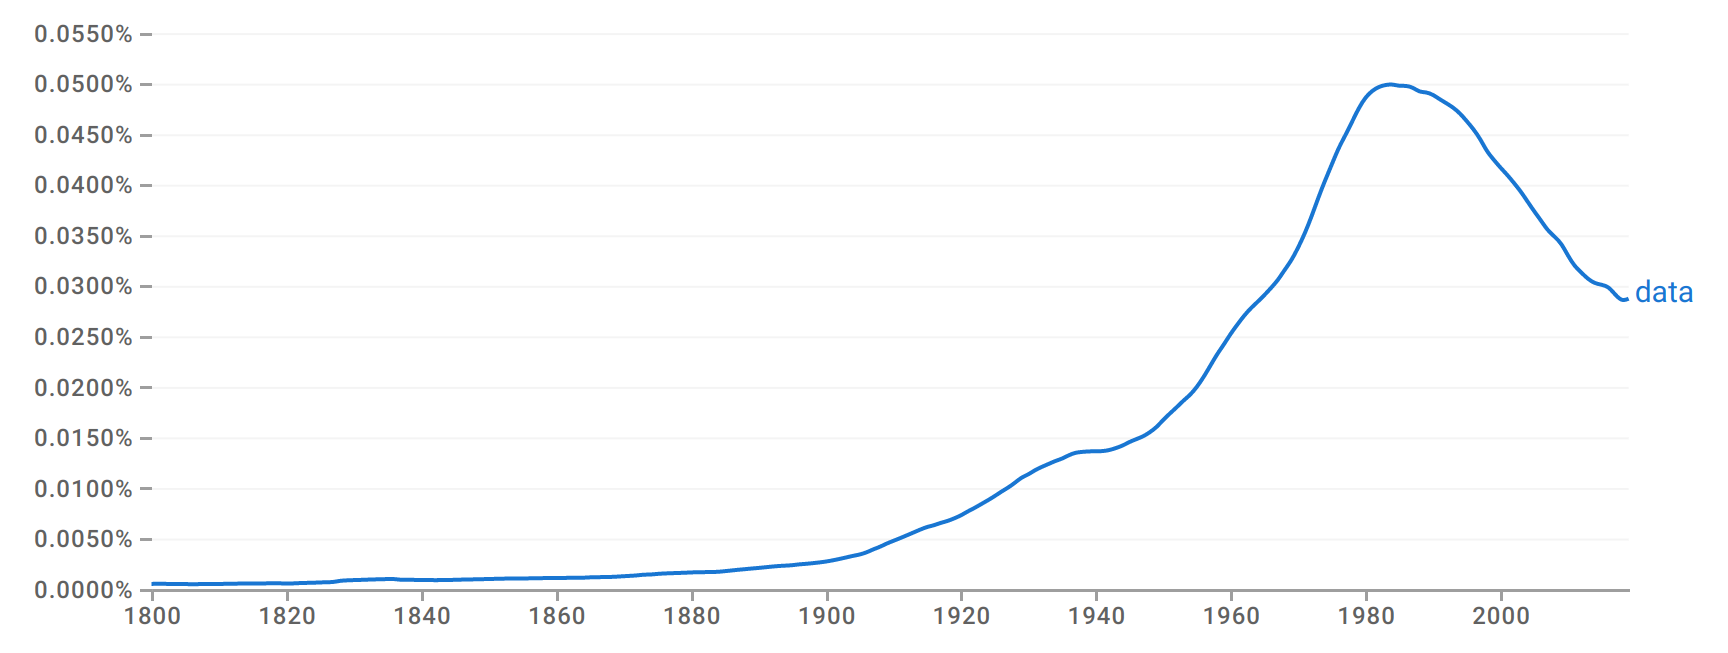
\includegraphics[width=\linewidth]{images/data-vocabulary-trend.png}
    \caption{英文书籍中单词“data”使用频率的变化,数据来自Google Book}
    \label{fig:data-trend}
\end{figure*}

\section{交通数据}

交通数据是指与交通系统的规划、设计、运营、控制相关的数据,是研究交通系统运行规律,解决现实交通问题的基础。本节概括介绍常见交通数据的类型、用途、获取方式。

交通最基本的定义是人和货物的移动;\emph{交通系统}是指人、货物、以及参与他们移动的其他要素的总和。
交通系统是由大量、相互作用的要素构成的复杂系统,为方便分析需要划分更小的子系统,由于交通系统的复杂性有多种划分标准,以下是几个例子:
\begin{itemize}
    \item 按照交通主体划分,可以分为客运交通和货运交通。
    \item 按照城市范围划分,可以分为市区交通和市郊交通,分别有不同的管理方式。
    \item 按照交通方式划分,某个区域的交通网络由道路、轨道、航空、水运、管道等子系统构成,分别有不同的技术特征、运营方式、适用条件。
    \item 按照经济角色划分,可以分为\emph{交通供应}和\emph{交通需求}两个部分,分别有不同的利益诉求\sidenote{例如供应方公交公司希望通过降低发车间隔来降低成本,需求方乘客希望增加发车间隔来减少等待时间}。
\end{itemize}
实际对交通系统的划分可以更加复杂。例如可以把以上三个标准任意组合,得到新的划分标准;也可以对划分后的子系统进一步划分。这里为了控制课程范围我们主要关注市区内基于道路和轨道的客运交通,简称\emph{城市交通}。该领域通常关注的数据将在以下小节分别介绍。

\subsection{路段交通状态数据}

路段交通状态数据是指路网中某个路段在某个时刻的交通流量、密度、速度数据,简称流密速数据。
简单来说,流量是单位时间通过给定道路断面的车辆数;密度是单位长度路段上某瞬间的车辆数;速度是指某个时间、空间范围内所有车辆轨迹的\emph{平均}速度。
路段是交通网络的最小组成部分,描述单个路段交通状态是分析整个路网交通状态的基础。

\subsubsection{流量调查}
路段流量数据的获取方式最简单,只需在路段某个位置记录通过车辆的数量。
传统方法是由调查人员在路边人工数车,这种方法的好处是不需要任何技术装备,因此2000年以前应用广泛。
人工调查的缺点是受人力成本的限制,调查规模小、数据采集速度慢、且难以做到全天侯全时段采集。

\begin{marginfigure}
    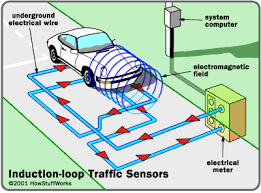
\includegraphics[width=\linewidth]{images/induction-loop-sensor.png}
    \caption{感应线圈检测器工作原理}
    \label{fig:induction-loop}
\end{marginfigure}

当前流量调查的主流方式时感应线圈检测器。该设备需要在路段地下埋设通电金属线圈,然后通过记录车辆压过线圈时产生的电磁感应电流脉冲来检测车辆,原理见\cref{fig:induction-loop}。该设备现在技术成熟、价格经济,已经普及到大城市的多数重要道路,成为最重要的交通数据来源。

\subsubsection{速度调查}

速度调查一般分为两个阶段,首先是单个车辆瞬时速度调查,然后是根据多个车辆的瞬时速度计算路段平均速度。单个车辆瞬时速度调查可以直接用测速枪,发射声波或电磁波,通过车辆反射波的多普勒效应推算车辆速度如\cref{fig:speed-gun}所示。
也可以用双断面法,测量车辆通过两个相邻断面的时间差,然后除以断面之间距离差来得到速度,如\cref{fig:section-speed}所示。

\begin{marginfigure}
    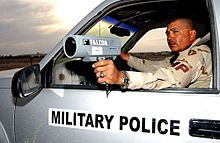
\includegraphics[width=\linewidth]{images/speed-gun.jpg}
    \caption{测速枪测速。}
    \label{fig:speed-gun}
\end{marginfigure}

\begin{marginfigure}
    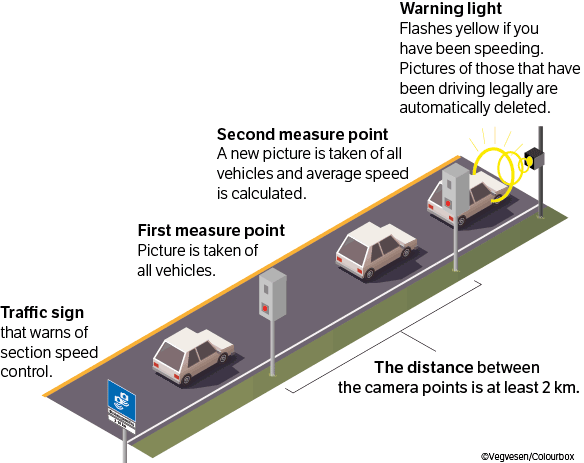
\includegraphics[width=\linewidth]{images/section-speed.png}
    \caption{双断面法测速。}
    \label{fig:section-speed}
\end{marginfigure}

\subsubsection{密度调查}
交通密度传统上一般难以直接调查,需要基于流量和速度间接推测。
交通密度直接调查需要进行高空俯视拍照,然后用照片范围内的车辆数除以路段长度就能得到交通密度。
为了保证照片的视野范围,拍摄站位一般需要飞机、热气球、高楼顶等高处,而实际上往往找不到合适位置,因此不可行。
另一方面流密速三者之间存在函数关系$q=k\cdot v$,同时流量$q$和速度$v$都比较容易获取,因此实际应用中一般通过$k=\frac{q}{v}$来推算密度。

\begin{figure}
    \sidecaption{路段车辆轨迹图;流量、密度、速度可以从轨迹推算。}
    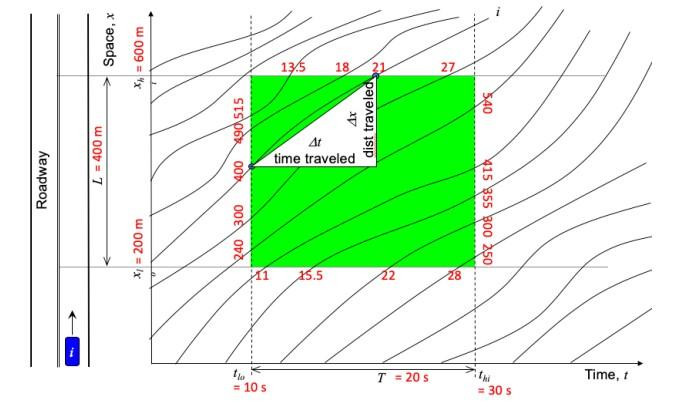
\includegraphics[width=\linewidth]{images/flow-density-speed.jpeg}
    \label{fig:trajectory}
\end{figure}
\subsection{车辆轨迹数据}
车辆轨迹数据又称车辆时空轨迹数据,是车辆时空位置记录构成的序列。每条记录记录包含两个成分,时间点和该时间点时车辆的空间位置;所有记录按时间点由早到晚排序。
一条车辆轨迹描述了某一车辆的完整活动轨迹,而车辆又是道路交通的最小单位,采集所有车辆的轨迹理论上可以掌握道路交通系统的完整状况。与路段流密速数据相比,车辆轨迹数据包含更加丰富的信息。从轨迹数据可以推算出流密速,反之则不成立,见\cref{fig:trajectory}。

车辆轨迹数据包含时间和位置两个成份,其中时间信息通过计时设备获取,比较简单,难点主要在空间位置信息的获取。
主要方式可以归纳为两类:路标定位和三角定位。

\subsubsection{固定信标定位}
设想你乘船在漆黑的大海上航行,如何获取自己的位置。
最简单的方法是去最近的灯塔,询问灯塔上的看守者。看守者知道自己灯塔的位置,你在这个灯塔附近因此也知道了自己的位置。在这个场景里灯塔这种位置已知的标记就是\emph{信标}。

在城市交通场景中可以承担信标角色的主要是固定的车辆身份识别设备,例如电子警察、ETC卡口等。
有车辆经过时这些设备能记录下车辆的身份、通过时间。
获取大量记录之后可以把某一辆车通过的卡口编号按时间顺序排列,然后将卡口编号替换为卡口位置,从而得到车辆的时空轨迹。
这种方法的核心是需要区分车辆的身份%
\sidenote{近年来兴起的所谓车路通信设备可以通过乘客手机上的蓝牙、Wifi信号区分乘客身份,进而间接区分车辆身份,因此也能作为固定信标。}%
,以免不同车辆的记录混淆,因此无法区分车辆身份的线圈检测器不能作为信标。

\subsubsection{三角定位}
固定信标定位简单易行,但有一个不足:只有到达信标附近才能用信标的位置来定位。
仍然以大海中的中的航船为例,航线中经过灯塔的时间和位置可以确定,而灯塔之间的实际航行路线无法确定,只能假设为直线。
要在不靠近灯塔的情况下确定船只位置需要用到附近至少三个灯塔,同时假设每个灯塔的位置已知,且有某种手段能测量船只和灯塔的距离。
每个灯塔的位置和距离把船只限定在一个灯塔的同心圆上,而三个灯塔同心圆的交点就是船只的位置。
这种获取位置的方法称为三角定位法,如\cref{fig:triangle-localization}所示。
\begin{marginfigure}
    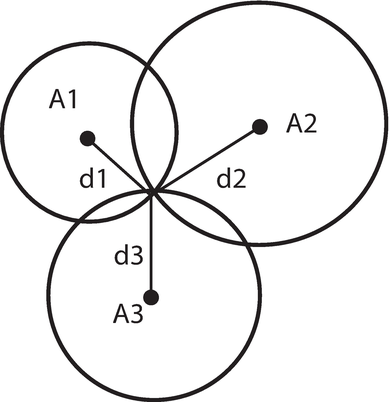
\includegraphics[width=\linewidth]{images/triangle-localization.png}
    \caption{三角定位法用三个固定信标推测当前位置。}
    \label{fig:triangle-localization}
\end{marginfigure}

在城市交通中常用的定位方式如卫星定位、手机基站定位本质上都是三角定位,只是担任信标角色的不是灯塔而是卫星和手机基站。
当前有几套卫星定位系统同时运行,包括美国的GPS系统、欧洲的伽利略系统、中国的北斗系统;其中GPS系统历史最长、覆盖范围最广。
几套系统的基本原理相似,天空中的卫星以固定轨道运行,位置已知,担任信标。
卫星持续向地面发射信号,信号中包含持续更新的高精度时间信息。
地面的定位设备接收卫星信号,比较信号的发射时间和接收时间,时间差乘以电磁波速度得到定位设备与卫星的距离。

手机基站定位原理类似,只不过用手机基站取代卫星作为电磁波发射源。
与卫星定位相比手机基站定位的精度低,而且只能在有手机信号的区域工作,覆盖范围窄。
但卫星定位与手机基站定位的最大区别在于前者是一种\emph{分散式}的数据采集手段,而后者是一种\emph{中心化}的数据采集手段。
设想我们要采集成都市所有人每天的活动轨迹。如果采用卫星定位技术,虽然现在所有手机都支持卫星定位但是我们很难让每一个手机用户都同意上传他的实时位置
\sidenote{现在有不少手机App会上传卫星定位数据到背后公司的数据库,如各种导航、点评、社交软件。}。
与之相对的是,如果采用手机基站定位,理论上只要运营商配合,不需要征得手机用户的同意就能获取成都所有人的实时位置。

\subsection{道路网数据}
道路网是城市交通最重要的基础设施,道路网数据是分析城市交通系统的基础数据。
道路网数据是城市地图数据的组成部分,一般包括道路平面位置和线型、车道划分、交叉口位置、交叉口渠化、交叉口信号控制方案等信息。
传统上道路数据的收集和处理主要属于地理信息专业,但现在随着智能交通的发展在交通专业中也越来越重要。

获取数字地图数据的方法主要是通过航拍、卫星图等方式获得某个区域的大范围照片,然后利用专业GIS软件在照片上描绘道路、房屋,并将各种信息输入数据库,如\cref{fig:gis-data-collection}所示。
传统上描绘过程需要人工操作,近年出现自动完成描绘的技术。
\begin{figure*}
    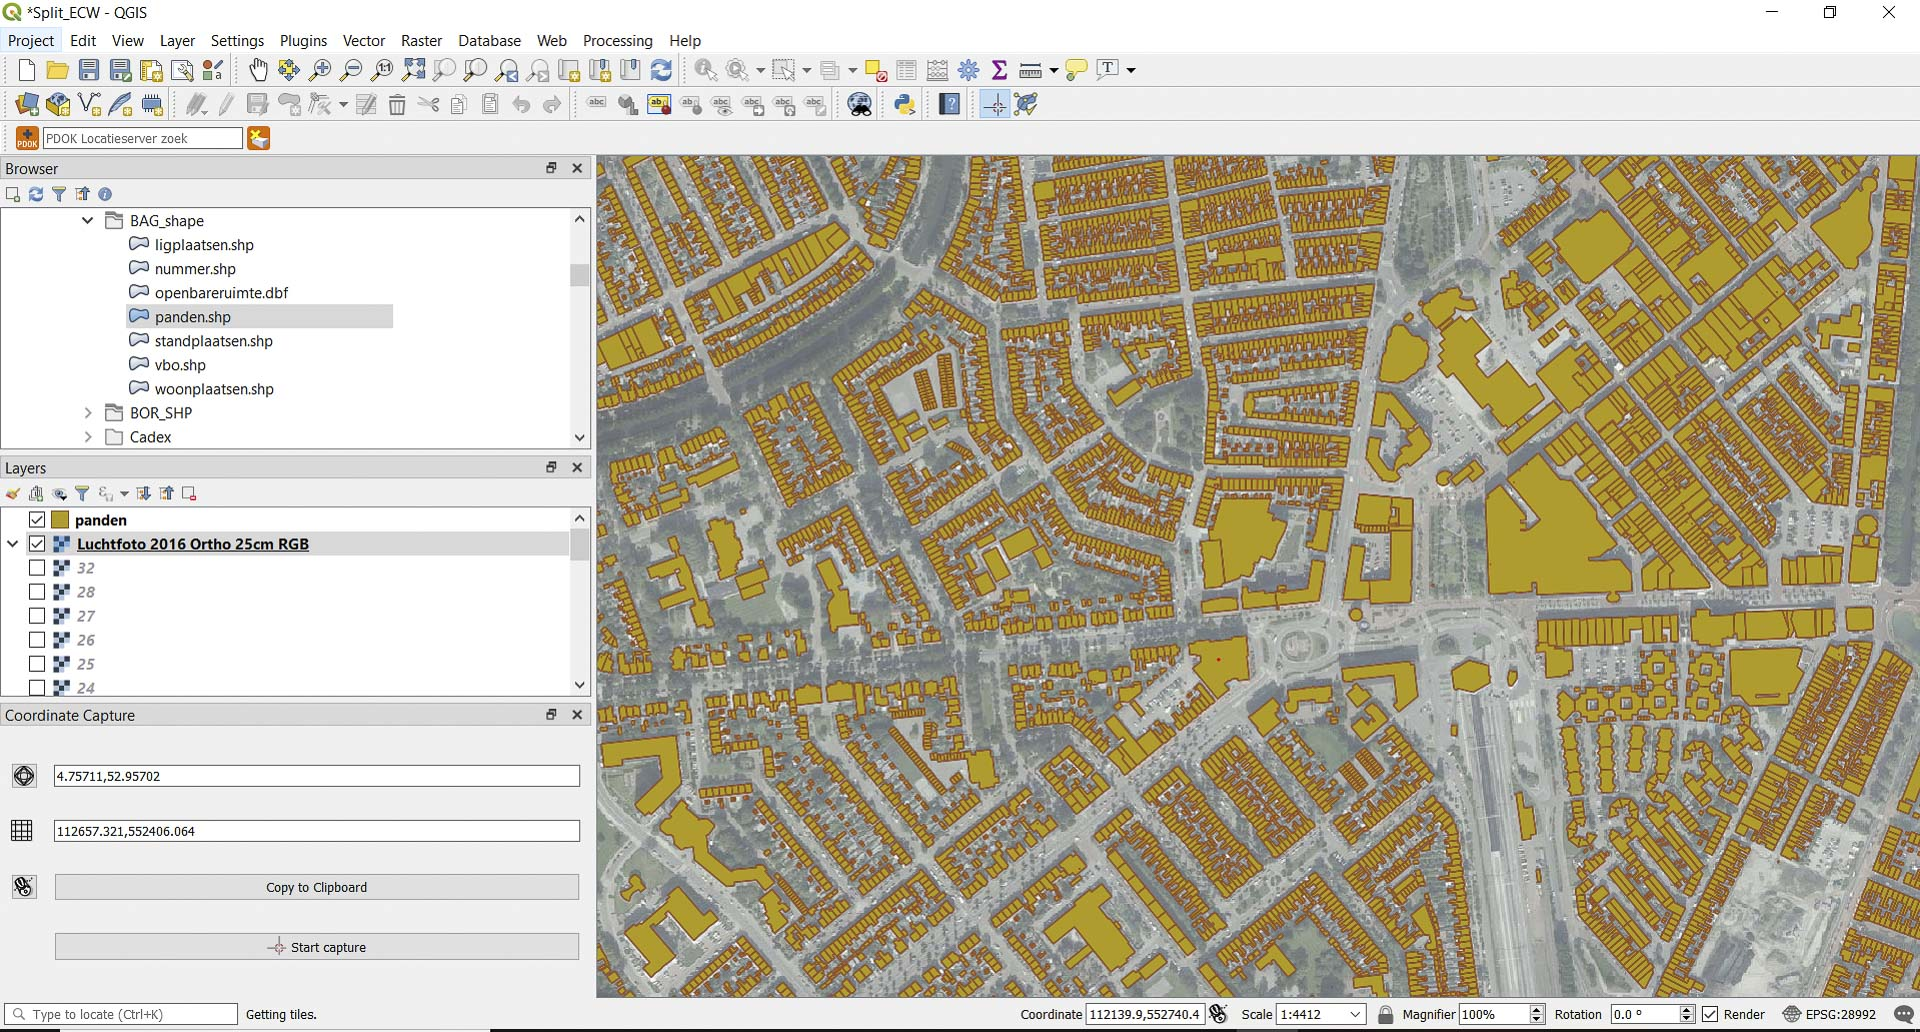
\includegraphics[width=\linewidth]{images/gis-data-collection.jpg}
    \caption{用QGIS软件处理卫星照片,建立数字地图数据}
    \label{fig:gis-data-collection}
\end{figure*}

\subsection{出行者行为数据}
之前的数据描述的是交通系统的状况,但解决交通问题往往需要探寻造成某种状况背后的原因。
决定交通系统状况最根本的原因是出行者的\emph{选择行为}。
每个出行者每天都面临着大到在什么地方买房定居、小到开车快慢的无数选择;
一个城市中所有出行者的所有选择共同决定了城市交通系统的状态。
例如大量出行者选择走某条道路会造成该道路拥堵,大量出行者同时去某个区域会造成该区域停车困难。

理解选择行为需要用到经济学模型,这些模型需要的数据包括出行者的社会经济背景,例如性别、年龄、收入、教育程度;各种偏好,例如时间和钱的兑换比例。这些数据一般通过问卷调查获取。

\section{什么是数据处理}

从各种渠道获取的数据称为\emph{原始数据},质量可能参差不齐,形式可能不符合要求,也可能太过繁杂难以抓住重点,因此需要经过处理才能变成有效的信息。
而\emph{数据处理}就是指用一切方法对数据进行变换,直到得到有效信息的过程。

数据处理的环节根据不同应用的要求多种多样,但以下这些环节比较常见。
\begin{description}
    \item[验证] 原始数据根据来源不同质量可能有很大差别。拿到数据后的第一步一般是验证数据质量,发现缺失、重复、错误、自相矛盾等问题,并力所能及的修正。如果修正不了至少要掌握误差的程度。
    \item[融合] 不同来源的数据往往有不同的形式,数据融合是将不同形式的数据统一到一个形式,方便后续使用。
    \item[统计] 大量细节数据容易造成信息过载,让人抓不住重点。通过统计手段可以将数据浓缩到少量关键值,例如均值、方差等,方便理解。
    \item[建模] 数据本身只反映出现象,重要的是探索现象背后的机理。综合利用各种数学工具可以建立数学模型,解释数据之间的关系,发现背后的机理。
    \item[可视化] 将数据从抽象的数字形式转化为图片、动画等可见的形式,利用人类视觉理解能力。通过可视化不只是方便展示数据处理的最终结果,更重要的是帮助发现数据中隐藏规律。
\end{description}
这些环节的内容后面章节都会涉及,但重点在数据建模上。